%%%%%%%%%%%%%%%%%%%%%%%%%%%%%%%%%%%%%%%%%%%%%%%%%%%%%%%%%%%%%%%%%%%%%%%%%%%%%%%%
%2345678901234567890123456789012345678901234567890123456789012345678901234567890
%        1         2         3         4         5         6         7         8

\documentclass[letterpaper, 10 pt, conference]{ieeeconf}  % Comment this line out if you need a4paper
\usepackage{graphicx}

%\documentclass[a4paper, 10pt, conference]{ieeeconf}      % Use this line for a4 paper

\IEEEoverridecommandlockouts                              % This command is only needed if 
                                                          % you want to use the \thanks command

\overrideIEEEmargins                                      % Needed to meet printer requirements.

%In case you encounter the following error:
%Error 1010 The PDF file may be corrupt (unable to open PDF file) OR
%Error 1000 An error occurred while parsing a contents stream. Unable to analyze the PDF file.
%This is a known problem with pdfLaTeX conversion filter. The file cannot be opened with acrobat reader
%Please use one of the alternatives below to circumvent this error by uncommenting one or the other
%\pdfobjcompresslevel=0
%\pdfminorversion=4

% See the \addtolength command later in the file to balance the column lengths
% on the last page of the document

% The following packages can be found on http:\\www.ctan.org
%\usepackage{graphics} % for pdf, bitmapped graphics files
%\usepackage{epsfig} % for postscript graphics files
%\usepackage{mathptmx} % assumes new font selection scheme installed
%\usepackage{times} % assumes new font selection scheme installed
%\usepackage{amsmath} % assumes amsmath package installed
%\usepackage{amssymb}  % assumes amsmath package installed

\title{\LARGE \bf
Advances in Robotic Learning Paper Summary: \\
Learning to Plan with Logical Automata
}

\author{Brandon Araki$^{1,*}$, Kiran Vodrahalli $^{2,*}$, Thomas Leech$^{1,3}$, Cristian-Ioan Vasile$^{1}$, Mark Donahue$^{3}$, Daniela Rus $^{1}$ \\
Presented by: Frank Liu, Evan Lam, Michael Drolet
\thanks{$^{1}$MIT CSAIL, Cambridge, MA 02139}% <-this % stops a space
\thanks{$^{2}$Columbia University, New York City, NY 10027 }%
\thanks{$^{2}$MIT Lincoln Laboratory, Lexington, MA 02421}%
\thanks{$^{*}$Authors contributed equally}%
}


\begin{document}



\maketitle
\thispagestyle{empty}
\pagestyle{empty}


%%%%%%%%%%%%%%%%%%%%%%%%%%%%%%%%%%%%%%%%%%%%%%%%%%%%%%%%%%%%%%%%%%%%%%%%%%%%%%%%
\begin{abstract}

This electronic document is a live template. The various components of your paper [title, text, heads, etc.] are already defined on the style sheet, as illustrated by the portions given in this document.

\end{abstract}


%%%%%%%%%%%%%%%%%%%%%%%%%%%%%%%%%%%%%%%%%%%%%%%%%%%%%%%%%%%%%%%%%%%%%%%%%%%%%%%%
\section{INTRODUCTION}
Recall the daunting time when you had to learn how to drive for the first time. In order to drive properly, you not only need to learn how to drive a car, but also learn the rules of the road. To learn how to drive a car, many of us practiced driving and learning all the mechanics to make the car move. Most of us went to a driving school, where a driving instructor taught us certain driving rules in the United States. Others might watch instructional videos from experts online. One way or another, we developed a mental model of the rules of the road through imitating an expert.
\newline
\indent Now there are two parts to this learning. The first part is learning the lower level actions in order to operate and drive a car. The second part is developing a mental model or representation of an interpretable policy, such as the rules of the road. The structure of the learned policy should be grounded in meaningful interpretations.
\newline
\indent When learning the rules of the road, a naive assumption is that all experts have taught properly and that all the instruction received is correct. If there are bad or even illegal driving habits, they will need to be corrected to ensure safe driving. For example, if a person runs a red light or makes an illegal u-turn, a police officer would reprimand and correct that behavior by issuing a ticket. We are able to be corrected because the rules in our heads are manipulable. Consequently, a human operator can easily modify a learned policy to perform similar but different policies. 
\newline
\indent Applying this to robot learning, the authors work toward teaching a robot to learn from demonstrations using not only a low-level policy, but also a high level policy that is interpretable and manipulable. The authors create a Logic-based Value Iteration Network (LVIN) which utilizes these two principles in learning policies. The policies that a robot learns should be interpretable, where there is a set of learned representation of rules. The behavior of the robot should be manipulable, where the rules can be changed in a predictable way which results in changed behavior. The LVIN model is a recurrent, convolutional neural network that uses value iteration over a learned Markov Decision Process (MDP). This MDP factors into two separate parts: a Finite State Automaton (FSA) corresponding to the low-level policy, as well as a bigger MDP corresponding to the rules in an environment.
\newline
\indent A major benefit to using this approach for learning is that a robot can both learn from demonstration and modify the learned policy to be safe. In the case of the driving example, if a robot was learning the rules of the road and five percent of the training data included illegal left turns (resulting in crashes), then the robot would learn the policy which crashes five percent of the time. With the author's approach in robotic learning, such a policy can be corrected to prevent crashes. These rules can also be applied in many alternative scenarios.
\newline
\indent In this paper, the authors main contributions are
\begin{enumerate}
  \item A Logic-based Value Iteration Network (LVIN) model that learns policies for robot learning from an imitation learning perspective. The authors show the effectiveness of the LVIN model through four different benchmark scenarios.
  \item Presenting that the model can learn transitions from state to state, therefore showing that it can interpret the rules.
  \item Demonstrating that the learning framework is manipulable, thus generalizable to other tasks and able to fix mistakes without extra training or experts.
\end{enumerate}

\section{Related Work}

\subsection{Logic-based Approaches}

Linear Temporal Logic (LTL) is a temporal logic language that is used to specify complex tasks which can then be translated into a finite state automaton (FSA). One work published in 2017 uses LTL to define the constraints on a Monte Carlo Tree Search for generating task plans to navigate through complex environments [3]. Other works have used LTL-derived FSAs in conjunction with MDPs to make reinforcement learning more efficient [4,5].

\subsection{Multitask and Meta Learning}

\begin{itemize}
  \item Learning many things at the same time.
  \item One shot learning.
\end{itemize}

\subsection{Faulty Experts}

\begin{itemize}
  \item Reinforcement learning through imperfect demonstrations
  \item Intention learning vs Imitation learning
\end{itemize}

\subsection{Hierarchical Learning}

\begin{itemize}
  \item Reinforcement learning through hierarchy of machines.
  \item Hierarchical Imitation and Reinforcement learning
\end{itemize}

\section{Problem Statement}
The overall goal is of this paper is to create a model that learns from demonstration a low-level policy, as well as a high level policy that is interpretable and manipulable. For our problem statement, we make a few assumptions. 
\begin{itemize}
  \item We assume that rules can be encoded as finite state automaton (FSA). 
  \item We assume that the relative features in an environment can be detected.
  \item We assume that the FSA states are known.
  \item We assume that the environment outputs current FSA state and low level state at each time step.
  \item The learned policy comes from the learned transitions among the FSA states and low-level transitions.
\end{itemize}

When authors say that they can detect the relative features of an environment, what they mean is that these features can be treated as logical propositions or a true/false variable. For example in a 2D grid environment, if there is a red light in the environment then at that particular grid position (x,y) where the red light is located the variable would be set to true. If there was no red light, then the variable would be set to false.
\newline
\indent We assume that the expert is following some sort of finite state controller. This finite state maps to the variables in the environment with different states corresponding to the variables environment. There are different actions based on the variable. For example, move forward on a green light as an action in the state machine. The FSA which the expert follows is the overall policy in which our network wants to learn. The learnt FSA is interpretable because the model can learn expert trajectories. Additionally, this model can obtain new policies without re-learning a changed expert FSA.

\subsection{Value Iteration Network} 
The LVIN network is based off of the Value Iteration Network [2]. The Value Iteration Network architecture is a fully differentiable version of value iteration. The Q function is calculated using a convolution and the Value function is calculated using a max pool function. This lets you learn the reward function and transition function. One limitation is that this Value Iteration Network is that it works best in a 2D grid environment due to the structure of the network.
\begin{figure}[h]
 \centering
 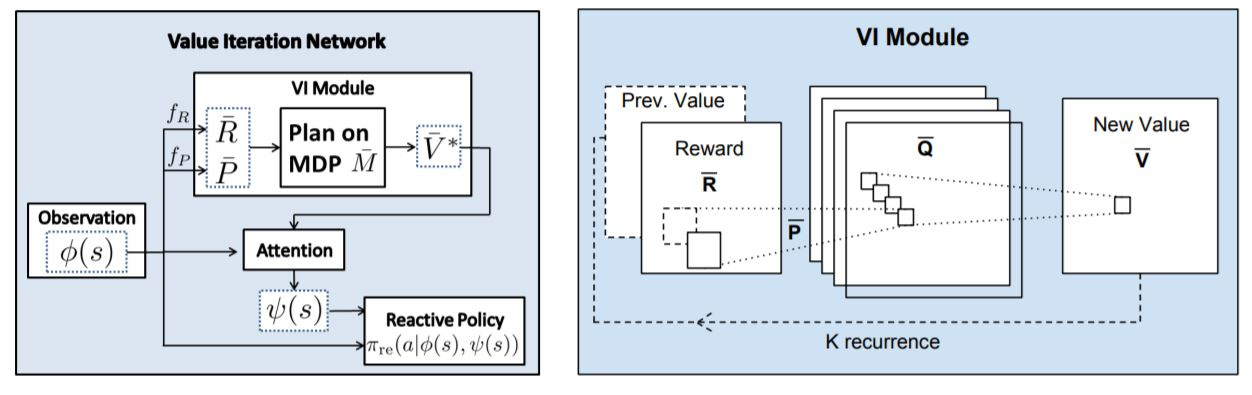
\includegraphics[scale=.33]{ValueIterationNetwork.JPG}\\
 \caption{A block diagram of the Value Iteration Network. The module is shown on the right. The reward function is R, while the transition function is P.}
\end{figure}
\newpage
\subsection{Logic-Based Value Iteration Network}
There are two differences between the Logic-Based Value Iteration Network and the Value Iteration Network. 
\begin{figure}[h]
 \centering
 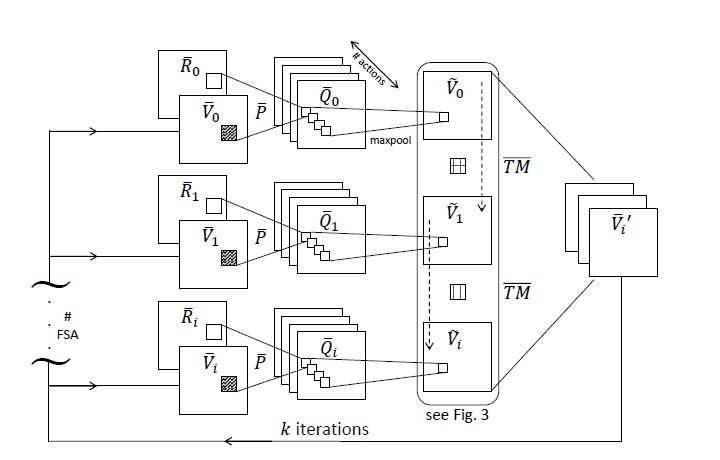
\includegraphics[scale=.5]{LVIN.JPG}\\
 \caption{A block diagram of the Logic-Based Value Iteration Network, figure 4 in the paper [1].}
\end{figure}

The first difference is that LVIN has a Value Iteration Network for every FSA state. As a result, the reward function and transition function are learned for every FSA state.
\newline 
\indent The second difference is there is a second convolution which is applied afterwards, which is represented by TM. This convolution is based off the transitions of the FSA. The second convolution helps the model learn the transitions of the FSA's.

\section{Experiments}
The LVIN model was tested against 2-3 baselines in 4 different virtual domains (Kitchen, Longterm, Pickworld, and Driving). Each domain emphasized a key claim of the LVIN network's capabilities. 

\subsection{Data Generation}

The authors use a software package to convert specified tasks into FSAs. Each FSA state contains a goal state, as well as undesired termination states. For each of the four domains, the authors generate proposition variables. The expert trajectories were created by using the Dijkstra's shortest path algorithm for the imitation learning data.

\subsection{Base Lines}

\begin{itemize}
  \item Value Iteration Network. The authors compared the LVIN to the VIN.
  \item Hard-coded LVIN. The TM is hard coded into the LVIN. The LVIN with a learned TM is compared to a Hard-coded LVIN with a known TM.
  \item CNN. Instead of a second convolution for the learned TM, there is a 3-D convolutional neural network attached at the end that learns the transitions of the FSAs.
\end{itemize}

\subsection{Domains}
\textbf{Kitchen}. In a 8x8 grid world in figure 3, the kitchen domain had milk, cereal and obstacles in the environment. The goal was to first fill a bowl with milk before filling it with cereal while avoiding the obstacles.
\begin{figure}[h]
 \centering
 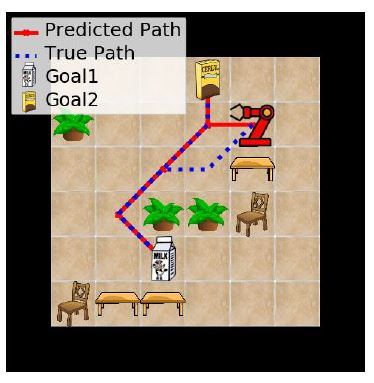
\includegraphics[scale=.6]{Kitchen.JPG}\\
 \caption{Kitchen Domain}
\end{figure}
Measuring the LVIN model against the baselines, we see in figure 4 that the LVIN model performs just as well as the hard-coded LVIN and CNN while the VIN performed poorly.
\begin{figure}[h]
 \centering
 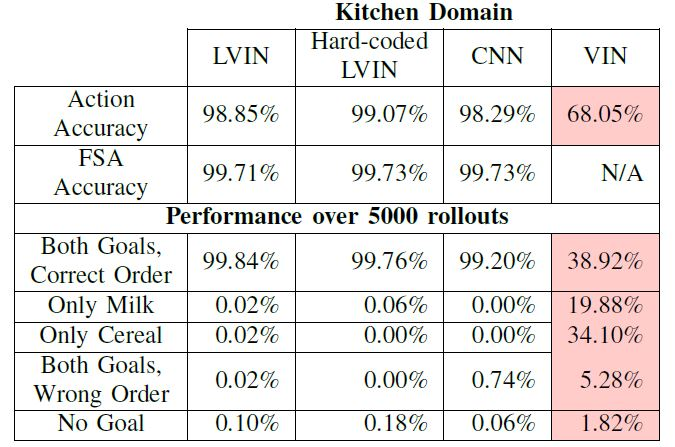
\includegraphics[scale=.6]{KitchenResults.JPG}\\
 \caption{Performance in the Kitchen domain}
\end{figure}
\newline
\textbf{Longterm}. In the 12x9 grid world in figure 5, the goal is to pick up each key to access the corresponding door to reach the goal position. This emphasizes learning long term complex behavior to reach the goal.
\begin{figure}[h]
 \centering
 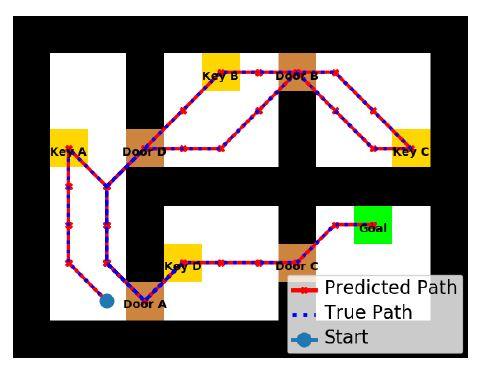
\includegraphics[scale=.5]{Longterm.JPG}\\
 \caption{Longterm Domain}
\end{figure}
\newpage
We see that the LVIN and CNN have good accuracy while the VIN struggles to learn the complex paths.
\begin{figure}[h!]
 \centering
 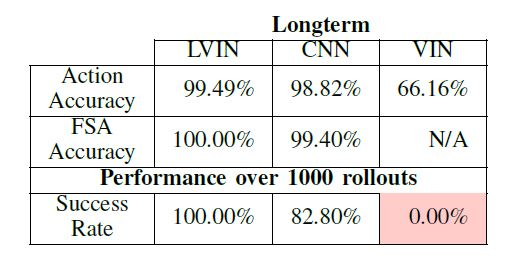
\includegraphics[scale=.6]{LongtermResults.JPG}\\
 \caption{Performance in the Longterm domain}
\end{figure}
\newline
\textbf{Pickworld}. In a 18x7 grid world in figure 7, the goal in the Pickworld domain is to first pick up either a sandwich a or a burger b and put it in a lunchbox d, and then pick up a banana c and put it in the lunchbox d.
\begin{figure}[h]
 \centering
 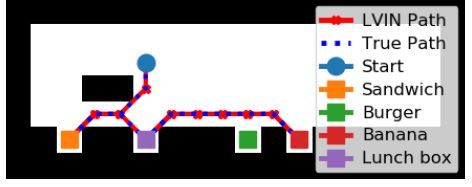
\includegraphics[scale=.5]{Pickworld.JPG}\\
 \caption{Pickworld Domain}
\end{figure}
The LVIN, the Hard-coded LVIN and the CNN performed the task quite well. The VIN struggled to learn the task. The LVIN models were the most successful.
\begin{figure}[h]
 \centering
 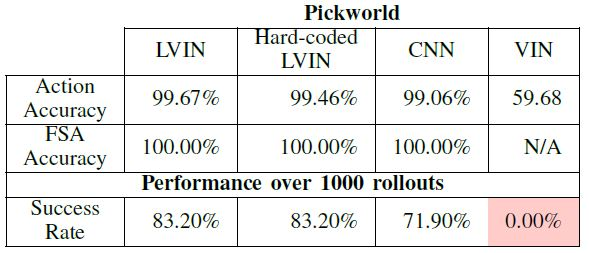
\includegraphics[scale=.6]{PickworldResults.JPG}\\
 \caption{Performance in the Pickworld Domain}
\end{figure}
\newline
\textbf{Driving}. In a 14x14 gridworld, this driving showcases the LVIN's ability to learn the rules of the world. The goal was to reach the goal position while learning to stop on red lights and wait until it turned green and to avoid obstacles in the environment.
\begin{figure}[h]
 \centering
 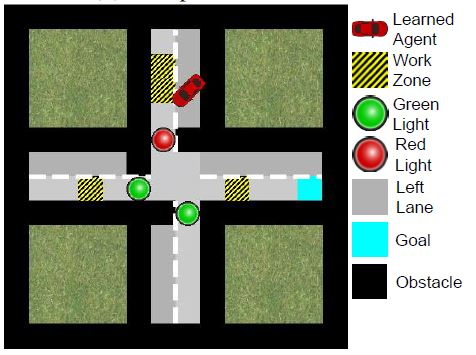
\includegraphics[scale=.5]{Driving.JPG}\\
 \caption{Driving Domain}
\end{figure}
Surprisingly, the VIN does better than the other baselines probably because there is only one sequential goal. LVIN, Hard-coded LVIN and CNN perform quite well.
\begin{figure}[h]
 \centering
 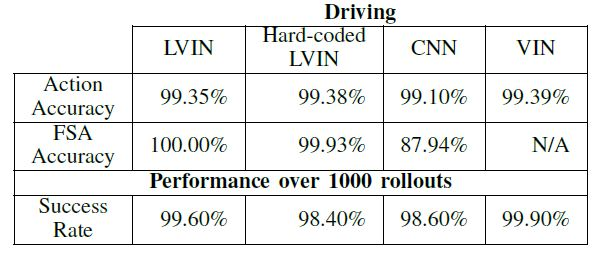
\includegraphics[scale=.6]{DrivingResults.JPG}\\
 \caption{Performance in the Driving Domain}
\end{figure}

\subsection{Interpretability and Manipulability Analysis}
\textbf{Interpretability}. Interpretability means that there is a meaningful learned FSA representations of rules. The learned TM should be similar to that of the true expert trajectory. We examine the different states and the corresponding learned TM and compare that with the true TM. Overall we see that the learned TM is similar to the true TM.
\newline
\newline
\textit{Kitchen}. For the kitchen, the goal of S0 is to reach goal a and S1 is to reach goal b.
\begin{figure}[h]
 \centering
 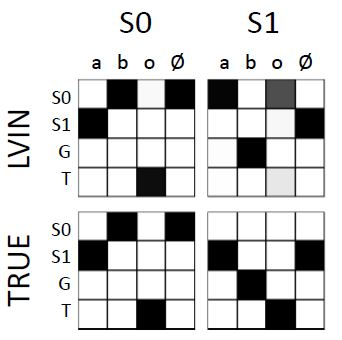
\includegraphics[scale=.6]{KitchenTM.JPG}\\
 \caption{Kitchen Transition Matrix}
\end{figure}
\newline
\textit{Pickworld}. For the Pickworld, the goal of S0 is to reach either a or b. The goal of S1 is to reach d. The goal of S2 is to reach c. The goal of S3 is to reach D again. The unexpected transitions are highlighted in red.
\newline
\begin{figure}[h]
 \centering
 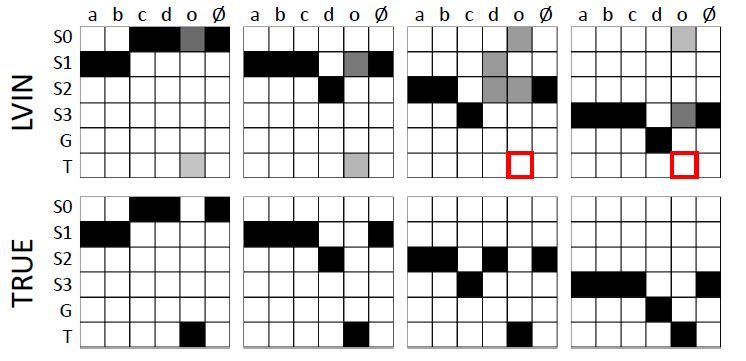
\includegraphics[scale=.4]{PickworldTM.JPG}\\
 \caption{Pick world Transition Matrix}
\end{figure}

\textit{Driving}. For the Drive world, the S0 is when the car drives on the right lane to reach the goal. S1 is when the car drives on the left lane to reach the goal. S2 is when the care is at a red light. The unexpected transitions are highlighted in red.
\begin{figure}[h]
 \centering
 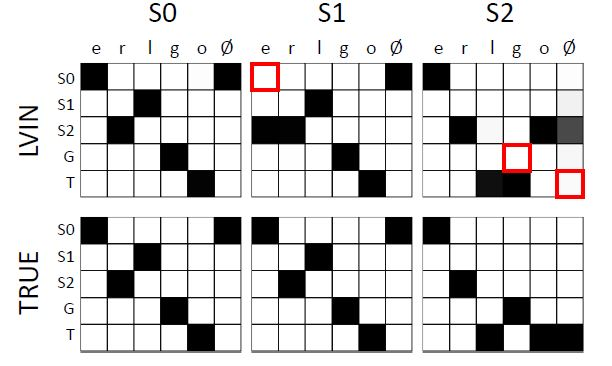
\includegraphics[scale=.5]{DrivingTM.JPG}\\
 \caption{Drive world Transition Matrix}
\end{figure}
\newline
\textit{Longterm}. For the Longterm world, there are far more states available compared to the other domains. There is a total of 10 propositions which map to 33 different states. One rule that confines the state space is that all the keys must be picked up in order as a result only 6 of the 33 possible states are visited. Each table is associated with a single state and shows how to get to the next FSA state.
\begin{figure}[h]
 \centering
 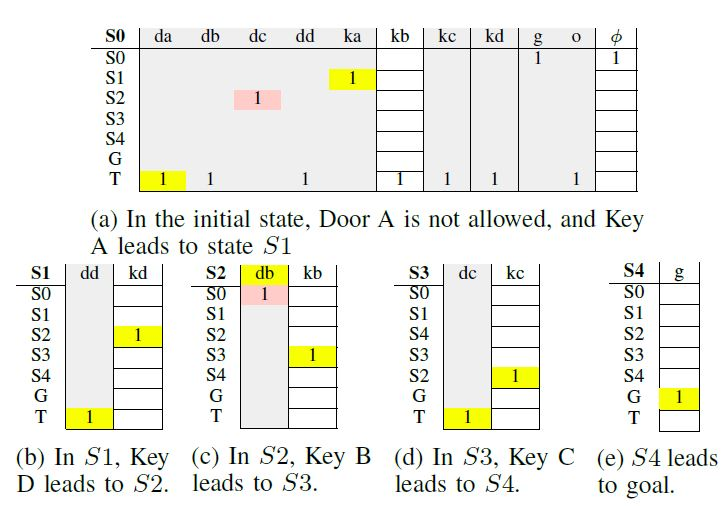
\includegraphics[scale=.45]{LongtermTM.JPG}\\
 \caption{Transition Matrix of the Long Term domain. The unvisited states are gray. The unexpected transitions are red. The cells of interest are in yellow.}
\end{figure}

\textbf{Manipulability}. Manipulability means that the behavior can be changed when the rules are modified in a predictable way which modifies the FSA transitions. The authors implement the pickworld domain onto a jaco arm to show the LVIN model working in real life. The objects were tracked with an optitracker and commands were sent via ROS. The transition matrix is modified for new behavior without relearning. 
\begin{figure}[h]
 \centering
 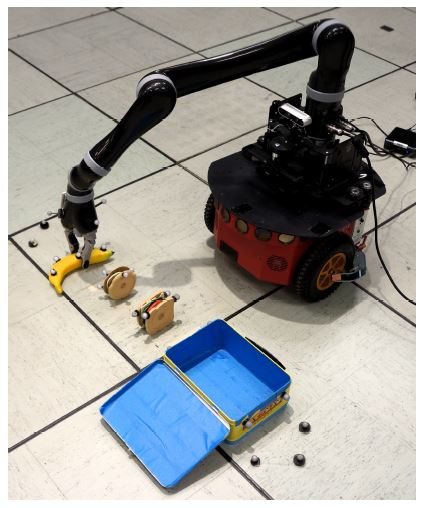
\includegraphics[scale=.3]{JacoArm.JPG}\\
 \caption{Pickworld with a Jacoarm.}
\end{figure}
\newpage
Below is the modified transition matrix with red representing deleted values and green representing added values. The authors use three different changed transition matrices to test.
\begin{figure}[h]
 \centering
 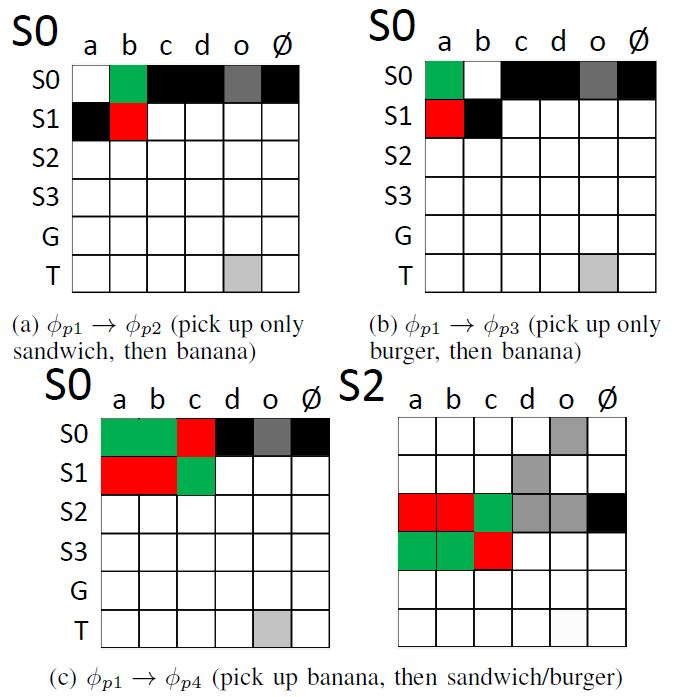
\includegraphics[scale=.5]{JacoArmTM.JPG}\\
 \caption{Modified transition matrix.}
\end{figure}

We saw that the performance of the LVIN, Mod. LVIN and the CNN were largely successful. The LVIN and CNN are baselines directly trained on the new specifications. The modified LVIN is the old LVIN with a changed transition matrix. The modified CNN did poorly because the TM is not included and the CNN performs the old specification. This highlights the need for manipulability which the LVIN is capable of. The failures resulted from the banana falling out the the jaco arm grip.
\begin{figure}[h]
 \centering
 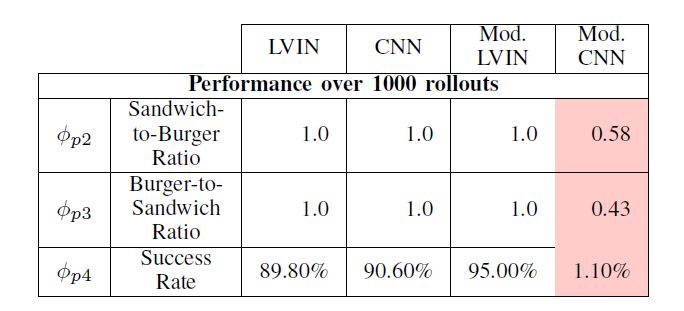
\includegraphics[scale=.5]{JacoArmResults.JPG}\\
 \caption{Jaco arm performance.}
\end{figure}
\begin{figure}[h]
 \centering
 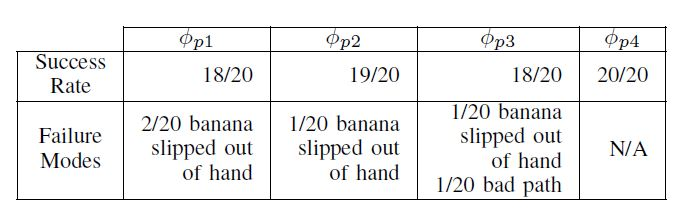
\includegraphics[scale=.5]{JacoArmFail.JPG}\\
 \caption{Reason for failure.}
\end{figure}

\section{Fixing Expert Mistakes}
Sometimes the data that is learned has a mistake. In this case, the authors used the driving world and had an issue of running a red light 10 percent of the time. The authors corrected this by setting the initial state entry to 0 and red light state entry to 1 to show there is a red light there. 
\begin{figure}[h]
 \centering
 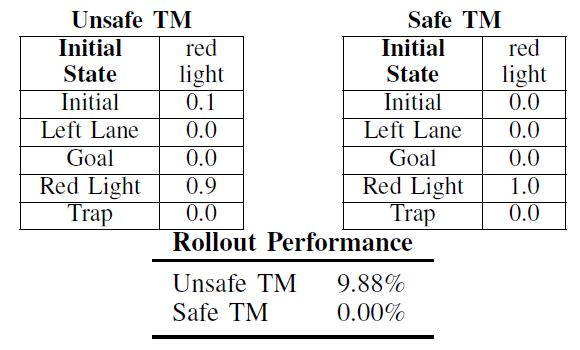
\includegraphics[scale=.5]{DrivingSafe.JPG}\\
 \caption{Safety driving scenario.}
\end{figure}

\section{Discussion and Analysis}
The authors mentioned was that the LVIN model works for finite grid world environments. These finite grid world environments are limited to a 2D grid. These applications might be incredibly useful integrated into a factory workplace with robots in highly controlled environments.
\newline
\indent However, the real world is three dimensional and highly unpredictable. These finite grid world environment limits LVIN's real world use case. While the authors have a real world experiment with the Jaco arm to show the LVIN model's effectiveness, the real world experiment exists in a highly controlled environment which is not representative of real world situations.
\newline
\indent A logical next step could be extending the 2D grid into a 3D grid world. We would imagine that the larger MDP for the rules of the world would add another dimension and the smaller FSA would add more states. Overall the new network model would be more complex. While the complexity of the network would increase, we do not believe the complexity change would not be too big of a problem in training on modern computers which train significantly large machine learning models.
\newline
\indent It also seems the manipulability of the learning is limited. The authors modify the state after detecting an error and to correct bad behavior. It would be quite interesting to see if the model can automatically detect errors and self correct. We imagine there can be neural network infrastructure which can be added for error detection.
\newline
\indent It would be quite interesting to explore the LVIN model with moving objects/obstacles in the 2D grid environment. How much would that effect the learned policies and how much impact would introducing such dynamic objects change the output behavior.


\section{CONCLUSIONS}

In conclusion, the authors introduce a Logic-Based Value Iteration network which can learn policies from imitation learning and demonstration. The authors tackle how to generalize a learned policy for a particular behavior to a larger set of tasks. Additionally, the authors address how to deal with incorrectly learned policies from incorrect demonstration. This network is a combination of a finite state automaton and a larger markov decision process. The LVIN network is a generalization of the Value Iteration Network, where the LVIN network learns the relevant transitions and creates a policy from the transitions of the FSA's. The key idea of the LVIN network is that a value iteration module is added to the end of a FSA and these modules get linked together. 
\newline
\indent The authors measure the LVIN network performance in four different virtual domains (Kitchen, Longterm, Pickworld, and Driving) and a real world implementation with a jaco arm. The LVIN model is shown to be accurate and effective in generalizing to new task specifications, and correcting errors. Future works can focus on expanding the model dimensionality for 3D scenarios and even self learn errors and dynamic objects in the world.

\addtolength{\textheight}{-12cm}   % This command serves to balance the column lengths
                                  % on the last page of the document manually. It shortens
                                  % the textheight of the last page by a suitable amount.
                                  % This command does not take effect until the next page
                                  % so it should come on the page before the last. Make
                                  % sure that you do not shorten the textheight too much.

%%%%%%%%%%%%%%%%%%%%%%%%%%%%%%%%%%%%%%%%%%%%%%%%%%%%%%%%%%%%%%%%%%%%%%%%%%%%%%%%



%%%%%%%%%%%%%%%%%%%%%%%%%%%%%%%%%%%%%%%%%%%%%%%%%%%%%%%%%%%%%%%%%%%%%%%%%%%%%%%%



%%%%%%%%%%%%%%%%%%%%%%%%%%%%%%%%%%%%%%%%%%%%%%%%%%%%%%%%%%%%%%%%%%%%%%%%%%%%%%%%

\begin{thebibliography}{99}

\bibitem{c1} Araki, Brandon \& Vodrahalli, Kiran \& Leech, Thomas \& Vasile, Cristian-Ioan \& Donahue, Mark \& Rus, Daniela. (2019). Learning to Plan with Logical Automata.
\bibitem{c2} Aviv Tamar, Yi Wu, Garrett Thomas, Sergey Levine, and Pieter Abbeel. Value iteration networks. In Advances in Neural Information Processing Systems 29, pages 2154– 2162, 2016.
\bibitem{c3} Chris Paxton, Vasumathi Raman, Gregory D Hager, and Marin Kobilarov. Combining neural networks and tree search for task and motion planning in challenging environments. ArXiv e-prints, 2017.
\bibitem{c4} Mohammadhosein Hasanbeig, Alessandro Abate, and Daniel Kroening. Logically-constrained reinforcement learning. arXiv preprint arXiv:1801.08099, 2018.
\bibitem{c5} Xiao Li, Yao Ma, and Calin Belta. Automata guided hierarchical reinforcement learning for zero-shot skill composition. ArXiv e-prints, 2017.


\end{thebibliography}




\end{document}
